% TEX compiler = latexmk
% copyright arturo salinas-aguayo 2024
\documentclass[12pt]{article}

\usepackage{graphicx}
\usepackage{amsmath}
\usepackage{array}
\usepackage{amsfonts}
\usepackage{fancyhdr}
\usepackage{geometry}
\usepackage{circuitikz}
\usepackage{subfigure}
\usepackage{caption}
\usepackage{karnaugh-map}
\usepackage{bm}
\usepackage{float}

\geometry{letterpaper, margin=1in}
\graphicspath{ {../images/} }

% Header and Footer
\pagestyle{fancy}
\fancyhf{}
\fancyhead[L]{CSE 2301 - Lab 07: Hamming Code}
\fancyhead[R]{\thepage}
\setlength{\headheight}{15pt}

\author{Arturo Salinas-Aguayo}
\title{Lab 07: Hamming Code}
% theorem set
\newtheorem{example}{Example}
% Example block environment
\newenvironment{examp}
{\vspace{0.5cm}
 \hrule
\vspace{0.5cm}
\begin{example}}
{\hrule
\vspace{0.5cm}
\end{example}}

\begin{document}
\newcommand{\closure}[2][3]{%
	{}\mkern#1mu\overline{\mkern-#1mu#2}}
\newcommand\ncoverline[1]{\mkern1mu\overline{\mkern-1mu#1\mkern-1mu}\mkern1mu}
% Title Page
\begin{titlepage}
	\centering
	\vspace*{3cm}
	\huge\textbf{Lab 07: Hamming Code}\\
	\vspace{5cm}
	\Large\textbf{Arturo Salinas-Aguayo}\\
	\normalsize
	CSE 2301: Principles and Practice of Digital Logic Design\\
	Dr. Mohammad Khan, Section 003L-1248\\
	Electrical and Computer Engineering Department
	\vfill
	
\includegraphics[scale=0.1]{uconnlogo}\\
	College of Engineering, University of Connecticut\\
	\scriptsize{Coded in \LaTeX}
	\vspace*{1cm}
\end{titlepage}
\section*{Theory}
\subsubsection*{What is a Multiplexor?}
A Multiplexor allows the designer to choose from several possible inputs based
on the value of a \textit{select} signal.
The output is selected by the select signal. For example, for a 4:1 MUX has four
data inputs and one output.
\begin{figure}[H]
	\center{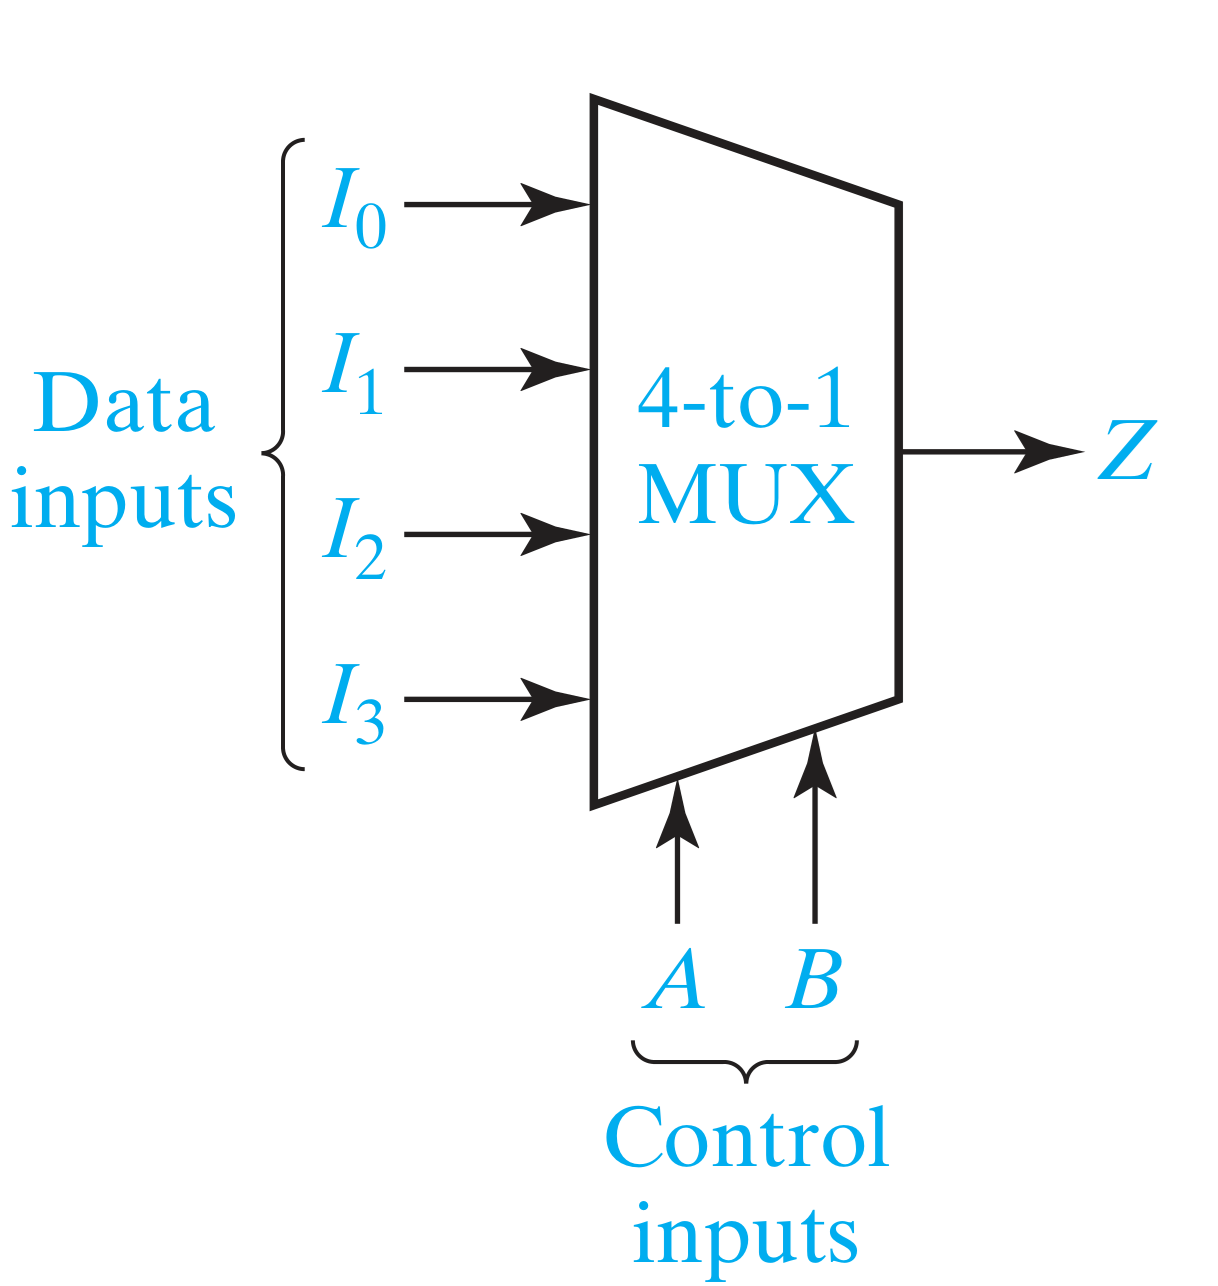
\includegraphics[scale=0.5]{examp081.png}}
	\captionof{figure}{4:1 MUX}
\end{figure}
Essentially, these IC's act as switches which select one of the inputs that is
connected to them. In general,

\textit{n} control inputs can be used to select one of \(2^n\) data inputs.
\[
	Z = \sum_{k=0}^{2^n-1} m_k \cdot I_k
\]
Where \(m_k\) is the k-th minterm of the select signals and \(I_k\) is the
respective data input.

The select lines can also be tied to a clock counter sort of signal in order to
cycle through the inputs. This is useful in analog circuits where a waveform can
be "compressed" into many cycles and decoded such that input 1 has a certain
frequency and amplitude and input 2 has another. This can introduce a lot of
noise however and makes it difficult to troubleshoot.

\subsubsection*{Why just half of a 74153?}
The lab has us design a circuit to implement two MUX's as a lookup table. In
this orientation, because each input MUX has two select states, and we only
utilize one output per MUX, we only need one of the two MUX's in the 74153.

Since we are using Shannon's expansion to convert the inputs to a function that
depends on the last input, each three person voting machine has select lines
assigned to two people, \(W\) and \(X\) in this case, and \(Y\) is used to be the
input to the mux as needed. By doing this, the inputs are limited to \(1, 0, Y
\) or  \(\overline{Y}\) and the output is a function of \(Y\).
\subsection*{Discussion}
\section*{Practice Questions}

\end{document}
% vim: set ft=tex tw=80 ts=2 sts=2 sw=2 noet:
